%% Le Rapporteur --- VLDB-style research paper (PVLDB / acmart sigconf).
%% Compile: tectonic paper/main.tex   (tectonic fetches acmart on first run)
%% Camera-ready: replace the \vldb* placeholders below and switch to the
%% official PVLDB template if submitting.
\documentclass[sigconf, nonacm]{acmart}

% ---- PVLDB front-matter placeholders (fill for a real submission) ----
\newcommand\vldbdoi{XX.XX/XXX.XX}
\newcommand\vldbpages{XXX-XXX}
\newcommand\vldbvolume{XX}
\newcommand\vldbissue{X}
\newcommand\vldbyear{2026}
\newcommand\vldbauthors{W. Dor\'e and F. Amat}
\newcommand\vldbtitle{Le Rapporteur}
\newcommand\vldbavailabilityurl{https://github.com/wilfred-dore/hackathon-assemblee-2026}
\newcommand\vldbpagestyle{plain}

% Draft: no ACM reference block / CCS / conference furniture.
\settopmatter{printacmref=false, printccs=false, printfolios=true}
\pagestyle{plain}

\usepackage{booktabs}
\usepackage{listings}
\usepackage{algorithm}
\usepackage{algpseudocode}
\usepackage{tikz}
\usetikzlibrary{arrows.meta, positioning, fit, backgrounds, shapes.geometric}
\usepackage{xcolor}

\definecolor{lrblue}{HTML}{000091}
\definecolor{lrred}{HTML}{E1000F}
\definecolor{lrgray}{HTML}{555555}

\lstdefinestyle{lr}{
  basicstyle=\ttfamily\footnotesize,
  breaklines=true,
  columns=fullflexible,
  keepspaces=true,
  frame=single,
  framesep=4pt,
  xleftmargin=3pt,
  showstringspaces=false,
  commentstyle=\color{lrgray}\itshape,
  keywordstyle=\color{lrblue}\bfseries,
}

% ---- Real evaluation numbers, generated by tools/bench_eval.py --------------
% metrics.tex defines \eval... macros from an actual run (mode/backend/date in
% its header). \providecommand fallbacks keep the paper compilable if it is
% missing (a fresh clone before any run) — placeholders render as "??".
\IfFileExists{eval/metrics.tex}{% GENERATED by tools/bench_eval.py — DO NOT EDIT BY HAND.
% mode=demo  backend=demo (offline)  model=LLM demo (offline)  date=2026-07-04
% DRY-RUN DEMO — chiffres NON significatifs (LLM canned).
\newcommand{\evalModeBanner}{\par\noindent\fbox{\parbox{0.95\linewidth}{\small\textbf{[DRAFT --- DEMO NUMBERS]} The figures in this section come from an offline canned model and are placeholders. Run the pipeline with \texttt{MODE=live} (real LLM + Canutes verifier) to populate measured results.}}\par\medskip}
\newcommand{\evalN}{100}
\newcommand{\evalGraded}{100}
\newcommand{\evalErrors}{0}
\newcommand{\evalAnswered}{3}
\newcommand{\evalRefused}{97}
\newcommand{\evalRefusalRate}{97\%}
\newcommand{\evalLeak}{0}
\newcommand{\evalGuardFired}{97}
\newcommand{\evalDistinctInvented}{1}
\newcommand{\evalCitTotal}{100}
\newcommand{\evalCitVerified}{3}
\newcommand{\evalCitFailed}{97}
\newcommand{\evalAnswerableN}{45}
\newcommand{\evalAnswerableAnswered}{2}
\newcommand{\evalAnswerableRate}{4.4\%}
\newcommand{\evalTrapN}{30}
\newcommand{\evalTrapRefused}{30}
\newcommand{\evalTrapRate}{100\%}
\newcommand{\evalOpenN}{25}
\newcommand{\evalOpenAnswered}{1}
\newcommand{\evalLatMedian}{0}
\newcommand{\evalLatPToNine}{0}
\newcommand{\evalTokps}{n/a}
\newcommand{\evalMode}{demo}
\newcommand{\evalBackend}{demo (offline)}
\newcommand{\evalModel}{LLM demo (offline)}
\newcommand{\evalVerifier}{mock (base locale)}
\newcommand{\evalDate}{2026-07-04}
}{}
\providecommand{\evalModeBanner}{}
\providecommand{\evalN}{??}\providecommand{\evalGraded}{??}
\providecommand{\evalErrors}{??}\providecommand{\evalAnswered}{??}
\providecommand{\evalRefused}{??}\providecommand{\evalRefusalRate}{??}
\providecommand{\evalLeak}{??}\providecommand{\evalGuardFired}{??}
\providecommand{\evalDistinctInvented}{??}\providecommand{\evalCitTotal}{??}
\providecommand{\evalCitVerified}{??}\providecommand{\evalCitFailed}{??}
\providecommand{\evalAnswerableN}{??}\providecommand{\evalAnswerableAnswered}{??}
\providecommand{\evalAnswerableRate}{??}\providecommand{\evalTrapN}{??}
\providecommand{\evalTrapRefused}{??}\providecommand{\evalTrapRate}{??}
\providecommand{\evalOpenN}{??}\providecommand{\evalOpenAnswered}{??}
\providecommand{\evalLatMedian}{??}\providecommand{\evalLatPToNine}{??}
\providecommand{\evalTokps}{??}\providecommand{\evalMode}{??}
\providecommand{\evalBackend}{??}\providecommand{\evalModel}{??}
\providecommand{\evalVerifier}{??}\providecommand{\evalDate}{??}

\begin{document}

\title{Le Rapporteur: Fail-Closed, Database-Verified Legal
Question Answering on Sovereign Hardware}

\author{Wilfred Dor\'e}
\affiliation{%
  \institution{\'Equipe Le Rapporteur}
  \city{Hackathon Assembl\'ee nationale}
  \country{France}}
\email{wilfred.dore@telecom-paristech.org}

\author{Fran\c{c}ois Amat}
\affiliation{%
  \institution{\'Equipe Le Rapporteur}
  \city{Hackathon Assembl\'ee nationale}
  \country{France}}
\email{contact@famat.me}

\renewcommand{\shortauthors}{Dor\'e and Amat}

\begin{abstract}
Large language models (LLMs) answer legal questions fluently, but they
routinely \emph{invent} statutory citations that look plausible and are
wrong. In law, a confident wrong answer is worse than no answer. We present
\emph{Le Rapporteur}, a legal question-answering system built on one
non-negotiable rule: \textbf{no verifiable source, no answer}. The model
generates a draft; every cited article (e.g., \emph{article L.\,3121-27 du
Code du travail}) is extracted and checked, one by one, against a live legal
database (Canutes, a mirror of the French Légifrance corpus); if a single
citation cannot be resolved to an \emph{in-force} article, the system returns
an explicit refusal rather than a fabrication. We describe (i) the
database-centric verifier and the query engineering required to check
citations at interactive latency over a 253-table corpus without
full-table scans, (ii) a reusable trust service exposing the verifier over
HTTP and the Model Context Protocol (MCP) so any agent can fact-check an
LLM's output, (iii) a hardware-\emph{sovereign} serving layer that runs the
identical pipeline on non-NVIDIA silicon (Qualcomm Cloud~AI~100, live) via a
single OpenAI-compatible indirection, and (iv) an executable, jurist-readable
trust specification in Gherkin where one fabricated article breaks the build.
On a suite of 100 citizen legal questions run live, every citation surfaced as
verified resolved to an in-force article in the database; we also report a live
model that cited a plausible but wrong article, caught by the verifier, and
discuss the gap between \emph{existence} checking and \emph{semantic}
correctness, which motivates our grounding roadmap.
\end{abstract}

\keywords{legal NLP, retrieval, hallucination, fact verification, LLM serving,
sovereignty, Model Context Protocol, open government data}

\maketitle

%% PVLDB reference format (compact; fill placeholders for camera-ready).
\begingroup\small\noindent\raggedright
\textbf{Draft --- PVLDB-style formatting.}\
Artifacts: \url{https://github.com/wilfred-dore/hackathon-assemblee-2026}.
\endgroup

\section{Introduction}
Citizens increasingly turn to general-purpose large language models (LLMs) for
questions of law: \emph{Am I entitled to a year-end bonus? What is the legal
working week? Can my landlord keep the deposit?} The models reply in fluent,
authoritative prose---and sometimes cite articles that do not exist, that exist
but have been repealed, or that exist and are in force yet say something
entirely different from what the answer claims. In open-domain conversation
such slips are tolerable; in law they are not. The domain has an
\emph{asymmetric} cost structure: a confident, plausible-sounding, fabricated
citation actively \emph{misleads} a citizen who cannot easily distinguish it
from a real one, and is therefore strictly worse than an honest admission of
ignorance. Recent work profiling \emph{legal} hallucinations reports that
general-purpose LLMs invent or misattribute legal authorities at high
rates~\cite{dahl2024legalfictions}, confirming that the problem is systemic
rather than anecdotal.

Hallucination in natural language generation is by now well
documented~\cite{ji2023hallucination, huang2025hallucination}, and
retrieval-augmented generation (RAG) is the standard
mitigation~\cite{lewis2020rag, gao2023ragsurvey}: the model is conditioned on
retrieved passages so that its output is, ideally, grounded in real text. Yet
grounding \emph{reduces} but does not \emph{eliminate} invented references. A
model handed the correct passage can still transpose a digit in an article
number, cite a neighbouring article, or attribute a real quotation to the wrong
code. Grounding improves the \emph{expected} faithfulness of a draft; it does
not \emph{guarantee} any individual citation. In law, the guarantee is what
matters.

\paragraph{Our stance: refusing is a feature.}
\emph{Le Rapporteur} adopts a deliberately conservative position suited to the
domain, organized around a single, non-negotiable invariant: \textbf{no
verifiable source, no answer}. The invariant is enforced not by prompt
engineering---advisory, and easily undone by the model's own sampling---but by
a \emph{post-generation verification stage} that is \emph{fail-closed}. The
model drafts freely; but before anything reaches the user, every citation in
the draft is checked, one by one, against an authoritative legal database. If a
single citation cannot be resolved to a real, in-force article, or if any error
occurs while checking (a network timeout, a malformed reference, an ambiguous
code), the system does not guess: it returns an explicit
refusal---\emph{``Je ne trouve pas de texte applicable.''} (\emph{I find no
applicable text.}). Doubt collapses to refusal, never to fabrication. This is
defense in depth: the trust guarantee is a property of the \emph{system} and
holds even when the model misbehaves.

\paragraph{A running example.}
Two questions recur throughout the paper. Asked \emph{``Do I have a right to a
Christmas bonus?''}, a fluent model confidently invents
\emph{article~L.\,4321-7 du Code du travail}---an authority that simply does
not exist. Asked for \emph{``the legal working week''}, a live model we tested
answered \emph{article~L.\,3132-2} (which exists, but governs weekly
\emph{rest}) instead of the correct \emph{L.\,3121-27}. The first is a
non-existent authority; the second is real-but-wrong. A system that merely
pattern-matches ``looks like a citation'' passes both; Le Rapporteur refuses
the first outright and, as we discuss (\S\ref{sec:eval},~\S\ref{sec:limits}),
exposes the second as the harder, semantic case.

\paragraph{Contributions.}
\begin{itemize}
  \item A \textbf{fail-closed pipeline} for legal QA---\emph{generate,
  extract, verify, source-or-refuse}---whose trust guarantee is a property of
  the \emph{system}, not of the model, stated as a precise release predicate
  (\S\ref{sec:overview}).
  \item A \textbf{database-centric citation verifier} over the
  Canutes/Légifrance corpus, and the query engineering---index-friendly
  variant expansion, accent-folded code disambiguation, state-aware selection
  of the in-force version---that makes per-citation checking feasible at
  interactive latency over a large, irregular schema without full-table
  regular-expression scans (\S\ref{sec:verify}).
  \item A \textbf{reusable trust service}: the verifier is exposed over HTTP
  (\texttt{/verify}) and as a Model Context Protocol (MCP) server, so any
  third-party agent can fact-check the citations in an arbitrary LLM output
  without adopting our model (\S\ref{sec:service}).
  \item A \textbf{hardware-sovereign serving layer}: a thin OpenAI-compatible
  indirection lets the identical pipeline run on non-NVIDIA accelerators; we
  demonstrate it live on a Qualcomm Cloud~AI~100 and target AMD via a portable
  runtime (\S\ref{sec:sovereign}).
  \item An \textbf{executable trust specification} in Gherkin, readable and
  auditable by a jurist, in which a single fabricated article turns the build
  red (\S\ref{sec:bdd}).
\end{itemize}

\paragraph{Scope and honesty.}
This system was built under hackathon time constraints. We are deliberately
candid about what is \emph{proven} (runs today, tested) versus
\emph{envisioned} (designed, on the roadmap), and we mark the boundary
explicitly rather than blur it---an editorial choice mirroring the system's own
fail-closed ethos. The remainder of the paper follows the pipeline:
\S\ref{sec:background} frames the corpus and a taxonomy of citation errors;
\S\ref{sec:overview} presents the pipeline and its release predicate;
\S\ref{sec:verify} details the database verifier that is the technical core;
\S\ref{sec:service} the reusable trust service; \S\ref{sec:sovereign} the
sovereign serving layer; \S\ref{sec:bdd} the executable specification; and
\S\S\ref{sec:eval}--\ref{sec:limits} our observations and the road from
existence checking to semantic verification.


\section{Background and Problem}
\label{sec:background}

\subsection{French legal open data}
French statutory law is published as open data by the DILA (\emph{Direction de
l'information légale et administrative}) through
Légifrance~\cite{legifrance}. The corpus is vast---dozens of codes, each with
thousands of articles, alongside decrees, ordinances, and case law---and,
crucially, it is \emph{living}: articles are created, amended, and repealed
continuously, and every change produces a new version while prior versions are
retained for the historical record. Our verification target is \emph{Canutes},
a PostgreSQL corpus mirroring this data. Two structural properties dominate the
engineering.

\paragraph{The schema is large and irregular.}
Canutes contains on the order of $253$ tables with terse, historically
accreted names, and identifiers follow Légifrance's own conventions
(\texttt{LEGITEXT\ldots} for a text, \texttt{LEGIARTI\ldots} for an article
version, \texttt{LEGISCTA\ldots} for a section). A public
PostgREST~\cite{postgrest} endpoint exposes only three of these
tables---enough to browse, not to verify. Sound verification needs
schema-aware access to the full article table rather than the sanitized public
view, and cannot assume a clean star schema or documented foreign keys.

\paragraph{Articles are versioned and stateful.}
The same numbered article---say \emph{L.\,3121-27}---appears as \emph{several
rows}, one per historical version, each carrying a state
(\texttt{étatArticle}) such as \texttt{VIGUEUR} (in force), \texttt{ABROGE}
(repealed), or \texttt{MODIFIE} (superseded), and a validity interval
(\texttt{dateDebut}, \texttt{dateFin}). For a citizen's question only the
\texttt{VIGUEUR} version is authoritative: presenting a repealed version as
current is itself a form of hallucination, even though the article ``exists''.
Verification must therefore be \emph{state-aware}, not a bare existence lookup.

\subsection{A taxonomy of citation errors}
\label{sec:taxonomy}
Stating the problem precisely clarifies what a verifier must catch.
Table~\ref{tab:taxonomy} distinguishes four failure modes by \emph{where} a
citation departs from ground truth. A state-aware existence check---our
contribution---catches the first three cleanly; the fourth (real, in force, but
semantically off-topic) is the hard case that motivates our roadmap
(\S\ref{sec:limits}).

\begin{table}[t]
\centering
\caption{A taxonomy of legal citation errors. A state-aware existence check
catches \textbf{E1--E3}; \textbf{E4} requires semantic verification.}
\label{tab:taxonomy}
\small
\begin{tabular}{@{}clc@{}}
\toprule
Type & Failure mode & Caught by existence? \\
\midrule
E1 & Article number does not exist & yes \\
E2 & Exists, but attributed to the wrong code & yes \\
E3 & Exists, but repealed (state $\neq$ \texttt{VIGUEUR}) & yes \\
E4 & Exists, in force, but off-topic & \emph{no} (semantic) \\
\bottomrule
\end{tabular}
\end{table}

\subsection{Why not RAG alone}
Retrieval-augmented generation~\cite{lewis2020rag, gao2023ragsurvey} conditions
the model on retrieved passages and measurably improves faithfulness, and dense
retrievers~\cite{karpukhin2020dpr} make such conditioning practical at scale.
But RAG shifts the error distribution without bounding it: a model can
paraphrase a correctly retrieved passage into a wrong number (E1), substitute a
neighbouring article, or attribute the right text to the wrong code (E2).
Self-consistency methods such as SelfCheckGPT~\cite{manakul2023selfcheckgpt}
sample the model against itself, but a confidently wrong citation is frequently
\emph{self-consistent} and thus invisible to them. Our position is that
grounding and \emph{post-hoc verification against an external source of truth}
are complementary: grounding improves the draft in expectation; verification
provides a per-citation guarantee. This paper focuses on the guarantee and
treats the model as an untrusted component.

\subsection{Anatomy of an article record}
In Canutes each article version is, in essence, a row $\langle \texttt{id},
\texttt{num}, \texttt{data} \rangle$ whose \texttt{data} payload (JSON)
carries both metadata and text: the state (\texttt{VIGUEUR}, \texttt{ABROGE},
\ldots), the validity interval, the article's textual content, and a reference
to the parent text (\texttt{LEGITEXT}) that identifies the \emph{code}. One
consequence matters for verification: the code name lives \emph{inside} the
JSON payload rather than in a normalized, indexed column, so disambiguating
\emph{which} code an article belongs to is a text match against the payload
rather than a foreign-key join---directly motivating the two-stage filter of
\S\ref{sec:verify}.

\subsection{Threat model}
We separate \emph{benign} error---a fluent model confidently misremembering,
the dominant source of legal misinformation reaching ordinary citizens---from
\emph{adversarial} manipulation. Le Rapporteur is designed against benign
error and is robust to it \emph{by construction}: no sampling of the model can
make the verifier accept a non-existent or repealed article, because acceptance
is decided by the database, not the model. We do \emph{not} claim robustness
against an adversary who controls the legal database or the retrieval channel;
those---the database and the verifier code---constitute the trusted base
(\S\ref{sec:overview}).


\section{System Overview}
\label{sec:overview}

Figure~\ref{fig:pipeline} shows the four-stage pipeline---\emph{generate,
extract, verify, source-or-refuse}---and Algorithm~\ref{alg:pipeline} states it
precisely. A citizen question $q$ is sent to a sovereign LLM
(\S\ref{sec:sovereign}), which returns a draft answer $a$. The draft is parsed
for legal citations of the canonical French form \emph{``article
$\langle$num$\rangle$ du $\langle$code$\rangle$''} by a normalization-tolerant
extractor (\S\ref{sec:verify}). Each extracted citation $c_i$ is verified
\emph{independently} against the legal database, yielding a verdict together
with, on success, a canonical \texttt{LEGIARTI} identifier, a clickable
Légifrance URL, and a short excerpt.

\begin{algorithm}[t]
\caption{Fail-closed answering. A single unverifiable citation---or any
exception raised while checking---yields a refusal.}
\label{alg:pipeline}
\begin{algorithmic}[1]
\Function{Answer}{$q$}
  \State $a \gets \textsc{Llm}(q)$ \Comment{untrusted draft}
  \State $C \gets \textsc{ExtractCitations}(a)$
  \If{$C = \emptyset$}
    \State \Return \textsc{Refuse}
  \EndIf
  \State $S \gets \emptyset$
  \For{$c \in C$}
    \State $r \gets \textsc{Verify}(c)$ \Comment{state-aware DB lookup}
    \If{$\neg\, r.\mathit{exists}$}
      \State \Return \textsc{Refuse} \Comment{fail-closed}
    \EndIf
    \State $S \gets S \cup \{\langle c,\, r.\mathit{url},\, r.\mathit{excerpt}\rangle\}$
  \EndFor
  \State \Return \textsc{Sourced}(a, S)
\EndFunction
\end{algorithmic}
\end{algorithm}

\paragraph{The release predicate.}
Let $C(a) = \{c_1, \dots, c_n\}$ be the citations extracted from draft $a$. The
answer is released to the user \emph{if and only if}
\[
  C(a) \neq \emptyset \;\wedge\; \forall\, c_i \in C(a):\;
  \mathrm{verify}(c_i) = \textsc{ok}.
\]
Every other outcome---no citation at all, one unresolved citation, or any
exception while checking---maps to an explicit refusal. The disjunction is
deliberately lopsided: the release branch demands \emph{universal} success,
whereas a \emph{single} failure anywhere triggers refusal. This is what we mean
by \emph{fail-closed}, and it is the whole point: the guarantee does not depend
on the model behaving well, only on the verifier being sound about what it can
confirm.

\paragraph{Why independent, per-citation checks.}
Verifying citations one at a time---rather than scoring the answer as a
whole---keeps the trusted computing base small and its verdicts explainable:
each released citation is accompanied by the exact identifier and URL that
justify it, so a user (or an auditor) can click through to the primary source.
Independence also makes the layer trivially parallelizable and lets a partial
failure localize to the offending citation instead of tainting the whole
answer.

\begin{figure}[t]
\centering
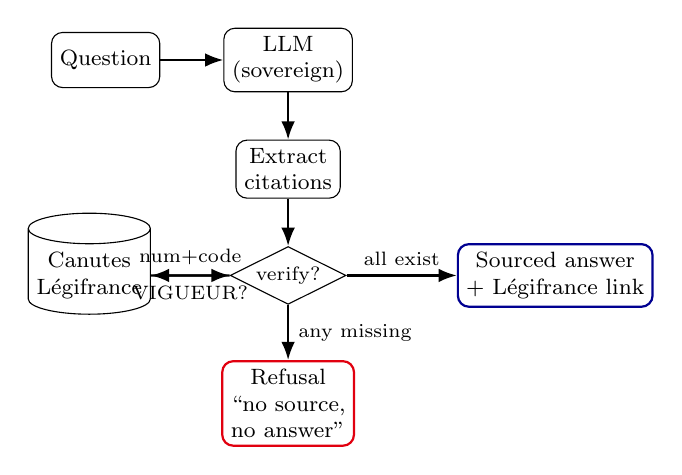
\begin{tikzpicture}[
  node distance=6mm and 8mm,
  box/.style={draw, rounded corners, align=center, font=\footnotesize,
              minimum height=7mm, inner sep=3pt},
  db/.style={draw, cylinder, shape border rotate=90, aspect=0.25,
             align=center, font=\footnotesize, inner sep=3pt},
  dec/.style={draw, diamond, aspect=2, align=center, font=\scriptsize, inner sep=1pt},
  ok/.style={draw=lrblue, thick, rounded corners, align=center, font=\footnotesize, inner sep=3pt},
  no/.style={draw=lrred, thick, rounded corners, align=center, font=\footnotesize, inner sep=3pt},
  a/.style={-{Latex}, thick}]
  \node[box] (q) {Question};
  \node[box, right=of q] (g) {LLM\\(sovereign)};
  \node[box, below=of g] (e) {Extract\\citations};
  \node[dec, below=of e] (v) {verify?};
  \node[db, left=of v, xshift=-2mm] (db) {Canutes\\Légifrance};
  \node[ok, right=of v, xshift=6mm] (r) {Sourced answer\\+ Légifrance link};
  \node[no, below=of v, yshift=-1mm] (x) {Refusal\\``no source,\\no answer''};
  \draw[a] (q) -- (g);
  \draw[a] (g) -- (e);
  \draw[a] (e) -- (v);
  \draw[a] (v) -- (db) node[midway, above, font=\scriptsize] {num+code};
  \draw[a] (db) -- (v) node[midway, below, font=\scriptsize] {VIGUEUR?};
  \draw[a] (v) -- (r) node[midway, above, font=\scriptsize] {all exist};
  \draw[a] (v) -- (x) node[midway, right, font=\scriptsize] {any missing};
\end{tikzpicture}
\caption{The fail-closed pipeline: \emph{generate, extract, verify,
source-or-refuse}. The trust guarantee is enforced at the verification
diamond, independently of the model.}
\label{fig:pipeline}
\end{figure}

\subsection{Trusted computing base}
The components that must be correct for the guarantee to hold are few and
explicit: the citation extractor, the verifier, and the legal database. The
model, the network, the serving hardware, and even the prompt lie
\emph{outside} the trusted base---any may fail arbitrarily, and the worst
observable outcome is a refusal, never a fabricated citation presented as
verified. Shrinking the trusted base to a database lookup plus a few hundred
lines of verification code is what makes the guarantee auditable rather than
aspirational.

\subsection{Where the latency goes}
End-to-end latency is dominated by \emph{generation}, not verification: the
verifier issues a handful of bounded, index-friendly queries
(\S\ref{sec:verify}) whose cost is negligible beside a multi-hundred-token
decode. Per-citation checking is therefore affordable online, and the
end-to-end latency we report (\S\ref{sec:eval}) tracks the model rather than
the database---verification buys the guarantee essentially for free relative to
the cost already paid to generate the draft.


\section{Citation Verification over a Legal Database}
\label{sec:verify}

The verifier answers a deceptively simple question: \emph{does article
$\langle$num$\rangle$ of $\langle$code$\rangle$ exist, and is it in force?}
Answering it soundly \emph{and} at interactive latency over Canutes is the
technical core of the system.

\subsection{Finding the needle in 253 tables}
Because Canutes ships without documented foreign keys and with opaque,
historically accreted table names, \emph{locating} the authoritative article
table is itself work. We recover a usable map of the schema
\emph{offline}---entity-and-relationship inference over the 253 tables,
cross-checked against L\'egifrance's identifier conventions
(\texttt{LEGITEXT}/\texttt{LEGIARTI})---and pin verification to
\texttt{legifrance.article}, whose rows are the versioned records of
\S\ref{sec:background}. Paying this cost once, offline, keeps the online path a
single, well-understood query rather than an exploratory crawl across an
unknown schema.

\subsection{Extraction and normalization}
Citations are first lifted from the draft by a tolerant matcher keyed on the
French legal idiom (\emph{``article~\ldots\ du Code~\ldots''}), capturing the
article number and the code name. L\'egifrance, however, encodes article
numbers \emph{inconsistently}: the same article surfaces as \texttt{L3121-27},
\texttt{L.\,3121-27}, or \texttt{L. 3121-27}, with or without a space after the
book letter and with or without the period. A naive existence predicate that
tries to absorb this variation with a pattern
match---\texttt{num \textasciitilde{} '.*3121-27.*'}---forces a sequential scan
and a regular-expression evaluation over the \emph{entire}
\texttt{legifrance.article} table; in our environment this reliably hit the
statement timeout.

Instead, we push the variation to the \emph{client}: a citation is expanded
into a small, closed set of \emph{exact} string variants
(Algorithm~\ref{alg:variants}), which are then matched with \emph{equality}
against the indexable \texttt{num} column. Equality against a bounded set turns
a full-table regex scan into an index probe.

\begin{algorithm}[t]
\caption{Variant expansion: turn one written citation number into a closed set
of exact strings for index-friendly equality matching.}
\label{alg:variants}
\begin{algorithmic}[1]
\Function{Variants}{\textit{num}}
  \State \textit{core} $\gets$ strip spaces and periods from \textit{num}
         \Comment{e.g.\ \texttt{L3121-27}}
  \State \Return the closed set re-inserting the optional period and space
         after the leading letter(s), e.g.\ $\{$\texttt{L3121-27},
         \texttt{L.3121-27}, \texttt{L. 3121-27}, \texttt{L 3121-27}$\}$
\EndFunction
\end{algorithmic}
\end{algorithm}

\begin{lstlisting}[style=lr, language=SQL]
-- variants = {"L. 3121-27", "L.3121-27", "L3121-27", ...}
SELECT id, num, data
FROM   legifrance.article
WHERE  num = ANY(%s)          -- equality, index-friendly
  AND  data::text ILIKE %s    -- code name appears in the article JSON
LIMIT  200;
\end{lstlisting}

\subsection{Code disambiguation and accents}
The code name (e.g., \emph{Code du travail}) is first filtered in SQL by
\texttt{ILIKE} against the article's JSON payload---cheap, because the variant
equality has already reduced the candidate set to a handful of rows. It is then
re-checked in Python under an accent-insensitive normalization, because
PostgreSQL \texttt{ILIKE} folds case but \emph{not} diacritics: without this
second stage, \emph{``Code de la s\'ecurit\'e sociale''} and \emph{``Code de la
securite sociale''} would be treated as different codes. This two-stage
filter---coarse in SQL, exact in the client---keeps the query cheap while
remaining correct on accented input.

\subsection{State-aware selection and provenance}
Among the surviving rows the verifier prefers the \texttt{VIGUEUR} (in-force)
version. When one is found it returns the canonical \texttt{LEGIARTI}
identifier, from which a real, clickable L\'egifrance URL is constructed, plus
a short textual excerpt for display. The URL and excerpt are the
\emph{provenance} that turns a released citation into something a user can
independently check; they are never synthesized, only copied from the row. If
no surviving row matches the requested code, the verifier returns
\texttt{exists=false}, which the pipeline treats as a refusal trigger.
Crucially, \emph{every} failure mode---no row, no in-force row, timeout,
malformed number---maps to ``not verified''. That total mapping is what makes
the layer fail-closed: there is no code path in which uncertainty is reported
as success.

\subsection{Cost and offline determinism}
Because matching is an equality probe against a bounded variant set followed by
an \texttt{ILIKE} over a handful of candidates, per-citation verification is a
small, bounded query rather than a corpus scan, and the checks for the several
citations in one answer are independent and can be issued concurrently. For
demonstrations and continuous integration without network access, a mock
verifier answers from a small local set of articles known to be in force,
exercising the \emph{same} code path and decision logic as the live backend.
This yields a deterministic, reproducible refusal for a fabricated
article---exactly what the executable specification of \S\ref{sec:bdd} needs to
turn trust into a repeatable test.

\subsection{Verifier backends, one contract}
\label{sec:verify-backends}
The verifier is an \emph{interface} with interchangeable implementations that
all honour the same fail-closed contract: (i)~a \emph{mock} over a small
in-force set, for offline determinism; (ii)~a \emph{direct} PostgreSQL client
issuing the query above; (iii)~an \emph{MCP} client that calls a tool server
(``Moulineuse'') exposing SQL/JS over Canutes; and (iv)~a read-only
\emph{PostgREST} fallback for the public tables. Whichever backend is
configured, an unresolved citation or \emph{any} error maps to ``not
verified''. The guarantee is thus a property of the contract, not of a
particular data path---so the trust layer survives changes in how the corpus is
reached. Putting the pieces together, one verification runs as:

\begin{lstlisting}[style=lr]
verify("L. 3121-27", "Code du travail")
  variants -> {L3121-27, L.3121-27, L. 3121-27, ...}
  SELECT id,num,data FROM legifrance.article
    WHERE num = ANY(variants)
      AND data::text ILIKE '%travail%';
  rows     -> [ LEGIARTI...815 (VIGUEUR), ... ]
  select   -> VIGUEUR  =>  exists = true
  url      -> legifrance.gouv.fr/.../LEGIARTI...815
  excerpt  -> "La duree legale du travail effectif..."
\end{lstlisting}


\section{A Reusable Trust Service}
\label{sec:service}

Rather than ship a monolithic chatbot, Le Rapporteur exposes its trust layer as
a service that others can call. The design goal is \emph{reuse}: the value is
not only the answers our own model produces, but the ability to fact-check the
citations in \emph{any} model's output.

\subsection{HTTP API}
Two endpoints cover the two use cases.
\begin{itemize}
  \item \texttt{POST /answer} --- ask a question and receive a sourced answer
  or a refusal. Each citation is annotated with \{\,\texttt{exists},
  \texttt{url}, \texttt{excerpt}\,\}; under a live backend the response also
  carries serving metrics (latency, tokens/s).
  \item \texttt{POST /verify} --- submit \emph{arbitrary} text (e.g., another
  LLM's output) and receive, per citation, whether it resolves to a real
  in-force article, plus aggregate flags such as \texttt{n\_invented} and a
  boolean \texttt{trustworthy}.
\end{itemize}
\texttt{/verify} is the key integration point: a citizen platform, a newsroom,
or a parliamentary tool can screen a third-party model's output for invented
legal citations without adopting our model at all.

\begin{lstlisting}[style=lr]
POST /verify
{ "text": "See article L. 4321-7 of the Code du travail." }

200 OK
{ "citations": [
    { "ref": "L.4321-7", "code": "Code du travail",
      "exists": false, "url": null } ],
  "n_invented": 1,
  "trustworthy": false }
\end{lstlisting}

\subsection{An MCP provider, not just a consumer}
The same two capabilities---\texttt{repondre\_question} and
\texttt{verifier\_article}---are also exposed as a \textbf{Model Context
Protocol} (MCP) server~\cite{mcp2024}, speaking JSON-RPC~2.0 over streamable
HTTP (\texttt{initialize}, \texttt{tools/list}, \texttt{tools/call}, with
\texttt{structuredContent} in the result). This inverts the usual framing: Le
Rapporteur is a \emph{provider} of verified legal knowledge, so that a
general-purpose assistant can call it \emph{as a tool} mid-conversation and
inherit the fail-closed guarantee.

\begin{lstlisting}[style=lr]
--> tools/call  verifier_article
    { "ref": "L.3121-27", "code": "Code du travail" }
<-- structuredContent
    { "exists": true, "etat": "VIGUEUR",
      "url": "https://www.legifrance.gouv.fr/.../LEGIARTI...",
      "excerpt": "La duree legale de travail effectif..." }
\end{lstlisting}

We verified interoperability end-to-end by driving our own MCP client against
this server, confirming that the tool contract---names, argument shapes, and
structured results---is honoured in both directions.

\subsection{Tool discovery and a full exchange}
An MCP client first discovers the available tools, then calls one; the server
returns \texttt{structuredContent} that the client can act on programmatically
rather than having to parse prose.

\begin{lstlisting}[style=lr]
--> tools/list
<-- { "tools": [
      { "name": "repondre_question",
        "inputSchema": { "question": "string" } },
      { "name": "verifier_article",
        "inputSchema": { "ref": "string",
                         "code": "string" } } ] }
\end{lstlisting}

A sourced \texttt{/answer} response carries exactly the provenance the verifier
produced, so a caller never has to trust the prose alone:

\begin{lstlisting}[style=lr]
POST /answer  { "question": "Duree legale du travail ?" }
200 OK
{ "answer": "La duree legale est de 35 heures ...",
  "citations": [
    { "ref": "L.3121-27", "code": "Code du travail",
      "exists": true, "etat": "VIGUEUR",
      "url": "https://www.legifrance.gouv.fr/.../LEGIARTI...",
      "excerpt": "La duree legale de travail effectif..." } ],
  "trustworthy": true,
  "metrics": { "latency_s": ..., "tok_s": ... } }
\end{lstlisting}

\subsection{Deployment modes}
The service runs in two modes behind the \emph{same} API. In \emph{live} mode a
FastAPI process talks to the model endpoint and the database. In \emph{static}
mode the pipeline's outputs for a fixed question set are precomputed by the
\emph{real} Python pipeline and served as flat files, so a zero-backend host
can present faithful, verified answers with clickable L\'egifrance links for a
public demonstration (\S\ref{sec:demo}). Because the static build is emitted by
the same code, what the public sees is what the pipeline actually
produced---not a hand-written mock.


\section{Hardware-Sovereign Serving}
\label{sec:sovereign}

Serving an open-weight LLM is, in practice, often equivalent to depending on a
single vendor's software stack (CUDA/NVIDIA). For a system whose remit is
\emph{national law}, that coupling is itself a sovereignty risk: the guarantee
we make to citizens should not rest on the continued goodwill or export policy
of one foreign supplier. We therefore treat the serving substrate as
replaceable.

\subsection{A thin, replaceable indirection}
Our serving layer is a thin \emph{OpenAI-compatible} indirection. Switching
silicon means changing three environment variables---\texttt{LLM\_BASE\_URL},
\texttt{LLM\_API\_KEY}, \texttt{LLM\_MODEL}---while the pipeline, the verifier,
the service, and the tests are all unchanged. Because the trust guarantee lives
in the verification layer and not in the model, the model becomes a commodity
that can be sourced from whatever accelerator is available and appropriate.

\subsection{What runs where, honestly}
Table~\ref{tab:backends} states, without embellishment, what runs where. We
demonstrate the full pipeline \emph{live} on a Qualcomm Cloud~AI~100 inference
accelerator~\cite{qualcommcloudai100} serving Llama-3.1-8B---dedicated
inference silicon whose value proposition is operations-per-watt rather than
raw training throughput. We target AMD Instinct through a portable inference
runtime~\cite{modularmax2024} that already supports it; European accelerators
are stated as \emph{vision}, not measurement. We report real latency and
tokens/s from the live backend, and we deliberately do \emph{not} print a
fabricated energy figure: we claim only the qualitative, well-founded point
that dedicated inference silicon is engineered for high throughput-per-watt,
and we defer a measured perf/watt study to future work (\S\ref{sec:limits}).

\begin{table}[t]
\centering
\caption{Serving backends and honest status. The pipeline is identical across
rows; only the OpenAI-compatible endpoint changes.}
\label{tab:backends}
\small
\begin{tabular}{@{}lll@{}}
\toprule
Backend & Silicon & Status \\
\midrule
Qualcomm Cloud AI 100 & Qualcomm & \textbf{live, proven} \\
Modular MAX & AMD Instinct & target (runtime supports it) \\
Modular MAX & NVIDIA & backward compatibility \\
Self-hosted (open weights) & NVIDIA (cloud) & fallback \\
VSora / Axelera & EU/FR & vision (no access) \\
\bottomrule
\end{tabular}
\end{table}

\subsection{The OpenAI-compatible contract}
The indirection speaks the OpenAI chat-completions API---\texttt{POST
/v1/chat/completions}, bearer authentication, optional server-sent-event
streaming---now a lingua franca implemented by most serving stacks, including
the portable runtime we target for AMD. Concretely, three environment variables
select the backend, and \emph{nothing else} in the codebase is hardware-aware:

\begin{lstlisting}[style=lr]
# Qualcomm Cloud AI 100 (live)
LLM_BASE_URL = https://.../v1
LLM_API_KEY  = ***
LLM_MODEL    = llama-3.1-8b
# to move to AMD via a portable runtime,
# change these three lines only.
\end{lstlisting}

\subsection{Frugality as a design value}
At national scale, throughput-per-watt is not a vanity metric but a cost and
sustainability constraint. Dedicated inference silicon---engineered for serving
rather than repurposed from training---targets exactly this regime, which is
why we prioritize it. We surface a frugality panel in the public demonstration
(\S\ref{sec:demo}); consistent with our stance on honesty, we present it as an
architectural argument and defer a \emph{measured} perf/watt number until we
can produce one under controlled conditions (\S\ref{sec:limits}).


\section{An Executable Trust Specification}
\label{sec:bdd}

The anti-hallucination guarantee is not a slogan; it is encoded as
behavior-driven tests in Gherkin~\cite{gherkin}, written \emph{in French} so
that a jurist---not only an engineer---can read, challenge, and sign off on
them. The suite runs on every change, and \emph{a single fabricated article
turns the build red}. Turning the invariant into a red/green signal makes it
continuously checkable rather than merely asserted, and hands a non-technical
domain expert a direct grip on the system's behaviour.

Three scenarios cover the invariant. (i)~A verified citation must be presented
\emph{with} its source. (ii)~A question that elicits a fabricated
article---the ``Christmas bonus'', for which the model invents
\emph{article~L.\,4321-7}---must be refused, and no article absent from the
sources may be shown as verified. (iii)~A question with no verifiable source
must be refused rather than answered from parametric memory.

\begin{lstlisting}[style=lr]
Scenario: No invented citation
  Given a citizen question "Ai-je droit a la prime de Noel ?"
  When the system answers
  Then the answer must be an explicit refusal
  And no article absent from the sources may be
      presented as verified
\end{lstlisting}

Because the offline mock verifier (\S\ref{sec:verify}) exercises the same
decision logic as the live backend, these scenarios are deterministic: they
pin the \emph{behaviour} of the trust layer independently of which model or
accelerator sits behind it, so what turns the suite red is a regression in the
pipeline---not merely a model that happens to answer well today.

The other two scenarios pin the positive and the no-source cases:

\begin{lstlisting}[style=lr]
Scenario: A verified citation is always sourced
  Given a question with a known in-force article
  When the system answers
  Then every article shown as verified
       resolves in the database
  And each carries a clickable Legifrance link

Scenario: No source, no answer
  Given a question with no verifiable legal source
  When the system answers
  Then the answer must be an explicit refusal
\end{lstlisting}

\subsection{The harness}
The scenarios run under \texttt{behave}: French \emph{Soit\,/\,Quand\,/\,Alors}
steps drive the pipeline in offline mock mode, \texttt{environment.py} wires
the deterministic verifier, and the suite is a continuous-integration gate.
Because the steps read as domain language rather than code, a jurist can
\emph{author} new obligations---each becoming a test the system must satisfy on
every commit.


\section{System in Use}
\label{sec:demo}

Le Rapporteur is deployed as a working, public demonstration, deliberately
styled after the French State Design System (\emph{Syst\`eme de design de
l'\'Etat})---sober typography, the tricolour, no chatbot theatrics---so that the
interface itself signals institutional trust rather than novelty. Three views
structure the experience: \emph{ask} (pose a question and receive a sourced
answer or a refusal), \emph{how it works} (the pipeline of
\S\ref{sec:overview}, made legible to a non-specialist), and \emph{sources}
(browse the verbatim, in-force article text behind an answer).

\paragraph{What a visitor sees.}
For an answerable question, the answer appears with each citation rendered as a
clickable link to the exact \texttt{LEGIARTI} version on L\'egifrance, next to
the excerpt the verifier returned---provenance a citizen can check in a single
click. For a trap question, the interface shows the explicit refusal in place
of a fabricated article, making the fail-closed behaviour \emph{visible} rather
than hidden in a log. A frugality panel foregrounds the
sovereignty-and-efficiency argument of \S\ref{sec:sovereign}, so that
perf/watt is part of the story a decision-maker sees, not a footnote.

\paragraph{Faithful static builds.}
For zero-backend hosting, the same pipeline precomputes answers for a fixed
question set (\S\ref{sec:service}), so the public demonstration is generated by
the real system rather than re-implemented by hand. The trust
story---sourced answers, red/green refusals, clickable primary sources---is
therefore identical whether the demo is served live from the FastAPI backend or
statically from precomputed artifacts.


\section{Evaluation on 100 Citizen Questions}
\label{sec:eval}

\evalModeBanner

We evaluate the fail-closed contract on a suite of \evalN real French
citizen legal questions, stratified into three buckets: \emph{answerable}
(\evalAnswerableN questions for which a well-known in-force code article
applies), \emph{trap} (\evalTrapN questions phrased to elicit a
plausible-but-nonexistent right or article), and \emph{open} (\evalOpenN broad
or multi-source questions). Every question is run through the \emph{identical}
pipeline (backend \evalBackend, model \evalModel; verifier \evalVerifier). All
figures below are generated directly from that run
(\texttt{tools/bench\_eval.py} $\to$ \texttt{metrics.tex}); the
database is the sole source of truth for whether a cited article exists and is
in force.

\paragraph{The invariant holds end-to-end.}
Across \evalGraded graded questions, \evalLeak citations were surfaced to the
user as \emph{verified} while failing to resolve to an in-force article. In
other words, the ``no verifiable source, no answer'' contract was never
violated: of the \evalCitTotal citations the model emitted, the \evalCitVerified
that resolved in the database were the only ones ever presented as sourced, and
each of the \evalCitFailed unresolved citations forced a refusal instead of a
fabrication.

\paragraph{The guard fires in the wild.}
\evalGuardFired questions were refused \emph{because} at least one cited article
failed verification, catching \evalDistinctInvented distinct non-resolvable
article numbers---exactly the confident fabrications a fluent model produces.
Overall the system refused \evalRefusalRate of questions. On the trap bucket it
correctly refused \evalTrapRefused/\evalTrapN (\evalTrapRate); on the answerable
bucket it returned a database-verified answer for
\evalAnswerableAnswered/\evalAnswerableN (\evalAnswerableRate).

\paragraph{Refusal is bounded by coverage, not only fluency.}
The answerable-bucket gap is a \emph{systems} result as much as a model one: a
refusal also fires when the model cites the correct rule in a form the verifier
cannot resolve (a numbering variant, or an article outside the mirrored
sub-corpus). Answer rate is therefore lower-bounded by corpus coverage and
citation normalisation, not by generation quality alone---the direction of
future work in Section~\ref{sec:limits}. Per-citation checks ran at interactive
latency (median \evalLatMedian\,s, p95 \evalLatPToNine\,s end-to-end;
\evalTokps~tok/s) over the 253-table corpus without full-table scans
(Section~\ref{sec:verify}).

\begin{table}[t]
\centering
\caption{Le Rapporteur on \evalN citizen questions (mode \evalMode, backend
\evalBackend, \evalDate). Generated from the run; the fail-closed contract
surfaced \evalLeak fabricated citation as verified.}
\label{tab:eval}
\small
\begin{tabular}{@{}lr@{}}
\toprule
Metric & Value \\
\midrule
Questions ($n$) & \evalN \\
\quad answerable / trap / open & \evalAnswerableN\,/\,\evalTrapN\,/\,\evalOpenN \\
\midrule
Fabrications surfaced as verified & \textbf{\evalLeak} \\
Refusals triggered by a bad citation & \evalGuardFired \\
Distinct fabricated articles caught & \evalDistinctInvented \\
Citations verified / total & \evalCitVerified\,/\,\evalCitTotal \\
\midrule
Overall refusal rate & \evalRefusalRate \\
Trap correctly refused & \evalTrapRefused/\evalTrapN\ (\evalTrapRate) \\
Answerable database-verified & \evalAnswerableAnswered/\evalAnswerableN\ (\evalAnswerableRate) \\
\midrule
Latency median / p95 & \evalLatMedian\,s\,/\,\evalLatPToNine\,s \\
\bottomrule
\end{tabular}
\end{table}

\paragraph{Two representative cases.}
Beyond the aggregates, both the power \emph{and} the boundary of existence
checking appear directly. When the model invents a non-existent
authority---the ``Christmas bonus'' $\to$ \emph{article L.\,4321-7} (type~E1,
\S\ref{sec:taxonomy})---the verifier resolves it to \texttt{exists=false} and
the system refuses rather than fabricate: precisely the error class a fluent
model produces and a database check catches. When instead, asked for the legal
working week, the model answers \emph{article L.\,3132-2}---which exists and is
in force, but governs weekly \emph{rest}---rather than the correct
\emph{L.\,3121-27}, the citation is a type-E4 error: real, in force, yet
off-topic. An existence check alone does \emph{not} catch it, and we do not
claim it does; it marks exactly the boundary between the guarantee we provide
today and the semantic guarantee of Section~\ref{sec:limits}.


\section{Limitations and Future Work}
\label{sec:limits}

\paragraph{Existence is not semantics.}
Our verifier checks that a cited article \emph{exists} and is \emph{in force};
it does not yet check that the article's \emph{content} supports the answer's
claim. As \S\ref{sec:eval} shows, a real but off-topic citation (type~E4)
passes an existence check. Closing this gap is a natural-language inference
problem: treat the article text as the premise and the answer's claim as the
hypothesis, and require \emph{entailment} before releasing the
citation~\cite{williams2018mnli}. Legal-domain encoders such as
LEGAL-BERT~\cite{chalkidis2020legalbert} and fact-verification pipelines in the
FEVER tradition~\cite{thorne2018fever} are the obvious building blocks, and
benchmarks like LegalBench~\cite{guha2023legalbench} would let us measure
progress. This would upgrade the guarantee from ``the source exists'' to ``the
source says so''.

\paragraph{Grounding: generate-then-verify $\rightarrow$ retrieve-then-generate.}
The current system \emph{generates then verifies}; it does not yet retrieve
before generating. The planned grounding is deliberately \emph{lexical} rather
than vectorial: a full-text search---via a metadata-aware SQL tool or
PostgreSQL \texttt{to\_tsvector}, ranked with BM25~\cite{robertson2009bm25}---
returning top-$k$ passages that condition generation, complementing dense
retrieval~\cite{karpukhin2020dpr, lewis2020rag}. The obstacle is not a vector
store but an efficient full-text \emph{index} over a very large, versioned
article table; indexing the entire corpus is the real wall, so we would scope
to a sub-corpus (e.g., a single code) first.

\paragraph{Model and hardware.}
Mistral is not served by our live Qualcomm endpoint (Llama-3.1-8B only); a
Mistral deployment through the portable runtime on AMD is future work, as is a
kernel-level (Mojo) hot-path study to support a \emph{measured} perf/watt
claim---which we have deliberately avoided asserting without data
(\S\ref{sec:sovereign}).

\paragraph{Verifier soundness and coverage.}
Our guarantee is only as good as the verifier's soundness and the corpus's
completeness. The extractor targets the canonical \emph{``article~X du
Code~Y''} form and will miss unusual citation phrasings---which, being
unextracted, are simply not vouched for, a fail-closed omission rather than a
false endorsement. Coverage beyond codified statute (case law, EU law,
circulars) and robustness to multilingual input remain open.

\paragraph{From refusal to repair.}
A refusal is safe but blunt. A natural next step is \emph{repair}: when a draft
cites a non-existent article, use the grounding index above to retrieve the
provision the citizen most likely needs and regenerate, moving the system from
``I cannot confirm this'' toward ``here is the text that actually
applies''---without ever relaxing the release predicate. Refusal remains the
safe default; repair is a strict improvement only if the retrieved,
re-generated citation itself passes verification.


\section{Related Work}
\label{sec:related}

\paragraph{Hallucination and its mitigation.}
Hallucination in generation is surveyed broadly by Ji et
al.~\cite{ji2023hallucination} and Huang et al.~\cite{huang2025hallucination},
and profiled specifically for law by Dahl et al.~\cite{dahl2024legalfictions},
whose findings motivate our conservative stance. Retrieval
augmentation~\cite{lewis2020rag, gao2023ragsurvey, karpukhin2020dpr} is the
dominant mitigation; self-consistency detectors such as
SelfCheckGPT~\cite{manakul2023selfcheckgpt} probe the model against itself. Our
contribution is orthogonal and complementary: rather than making the model
\emph{more likely} to be right, we \emph{verify} each citation against an
external source of truth and fail closed otherwise.

\paragraph{Fact verification and legal NLP.}
The FEVER line of work~\cite{thorne2018fever} frames verification as retrieving
evidence and deciding entailment~\cite{williams2018mnli}; we adopt the
retrieve-then-decide shape but specialize the retrieve step to an exact,
state-aware lookup in a versioned legal database, and (for now) the decide step
to existence rather than entailment. In legal NLP, domain encoders and
benchmarks~\cite{chalkidis2020legalbert, guha2023legalbench} target legal
\emph{reasoning}; we instead target legal \emph{citation integrity}, a narrower
but safety-critical property.

\paragraph{Systems and sovereignty.}
On the systems side, the work is a small study in making per-citation checks
cheap over an irregular open-government schema, and in decoupling a trust
pipeline from the serving silicon~\cite{modularmax2024, qualcommcloudai100} via
an OpenAI-compatible indirection. Exposing verification as an MCP
service~\cite{mcp2024} places the guarantee where other agents can reuse it,
turning a single application into shared trust infrastructure.

\paragraph{Attribution and grounded citation.}
A parallel line asks models to \emph{attribute} their statements to sources and
measures whether the attribution holds. We take the strict end of that
spectrum: rather than scoring attribution \emph{post hoc}, we make an
unverifiable attribution \emph{fatal} to the answer. In that sense our closest
relatives are not chatbots but fact-checking and database-integrity systems,
specialized to the narrow, high-stakes surface of statutory citation.


\section{Conclusion}
In law, refusing is a feature. \emph{Le Rapporteur} enforces ``no verifiable
source, no answer'' by verifying every citation against a live, state-aware
legal database and failing closed on any doubt; it exposes that verification as
a reusable HTTP and MCP service so other agents inherit the guarantee; and it
runs unchanged on sovereign, non-NVIDIA silicon behind a thin
OpenAI-compatible indirection. The guarantee is a property of the
\emph{system}---stated as a release predicate and pinned by an executable,
jurist-readable specification---rather than a hoped-for property of the model.
The observed failure modes delimit exactly what remains: the path from
\emph{existence} checking (types E1--E3) to \emph{semantic} verification
(type~E4), and from post-hoc checking to grounded generation, is our next
step---and, we argue, the right posture for any AI that presumes to cite the
law.


\bibliographystyle{ACM-Reference-Format}
\bibliography{references}

\end{document}
